\documentclass[a4paper]{article}

\usepackage{xcolor}
\usepackage[T1]{fontenc}
\usepackage{textcomp}
\usepackage{amsthm}
\usepackage{amsmath, amssymb}
\usepackage{enumitem}
\usepackage{transparent}
\usepackage[affil-it]{authblk}
\usepackage{graphicx}
\graphicspath{{./images/}}

\title{COMP 353 Databases\\
Assignment no.1}

\author{Duc Nguyen}
 \affil{Gina Cody School of Computer Science and Software Engineering \\
    Concordia University, Montreal, QC, Canada}
\date{Summer 2020}

\begin{document}
\maketitle

\newpage
\tableofcontents
\newpage

\section{Question 1 [Marks 50]}
\subsection{Problem Description}%

This problem involves an application where one needs to develop a relational database system
for a University. The following is the description of information available on the University:

\begin{itemize}
    \item Information on each department – name, location, and the employee working for the
department, programs offered, courses offered, and students enrolled.
    \item Information on each employee - employee ID, name, Social Security Number, title,
working department, salary, address, email address.
    \item Information on each faculty member – (in addition to employee’s information),
specialization, research area, research grants, students’ supervised, and courses taught
    \item Information on administrative personnel - (in addition to employee’s information)
qualification, special skills. 
    \item Information on each student – student ID, name, address, email address, program
enrolled-in, a detail list on courses (completed and/or registered with whom and termwise), and grades.
    \item Information on each graduate student – (in addition to student’s information) name of
supervisor, research topic, research fellowship (in terms of CND amount per year).
    \item Information on each course - course number, description, credit-hours
\end{itemize}
\newpage

\subsection{Part 1: Develop ER diagram}%
\label{sub:part_1_develop_er_diagram}
\textbf{Problem:}
Develop an ER diagram to represent the conceptual database scheme for the University.

\begin{figure}[h]
    \caption{Entity Relationship Diagram}
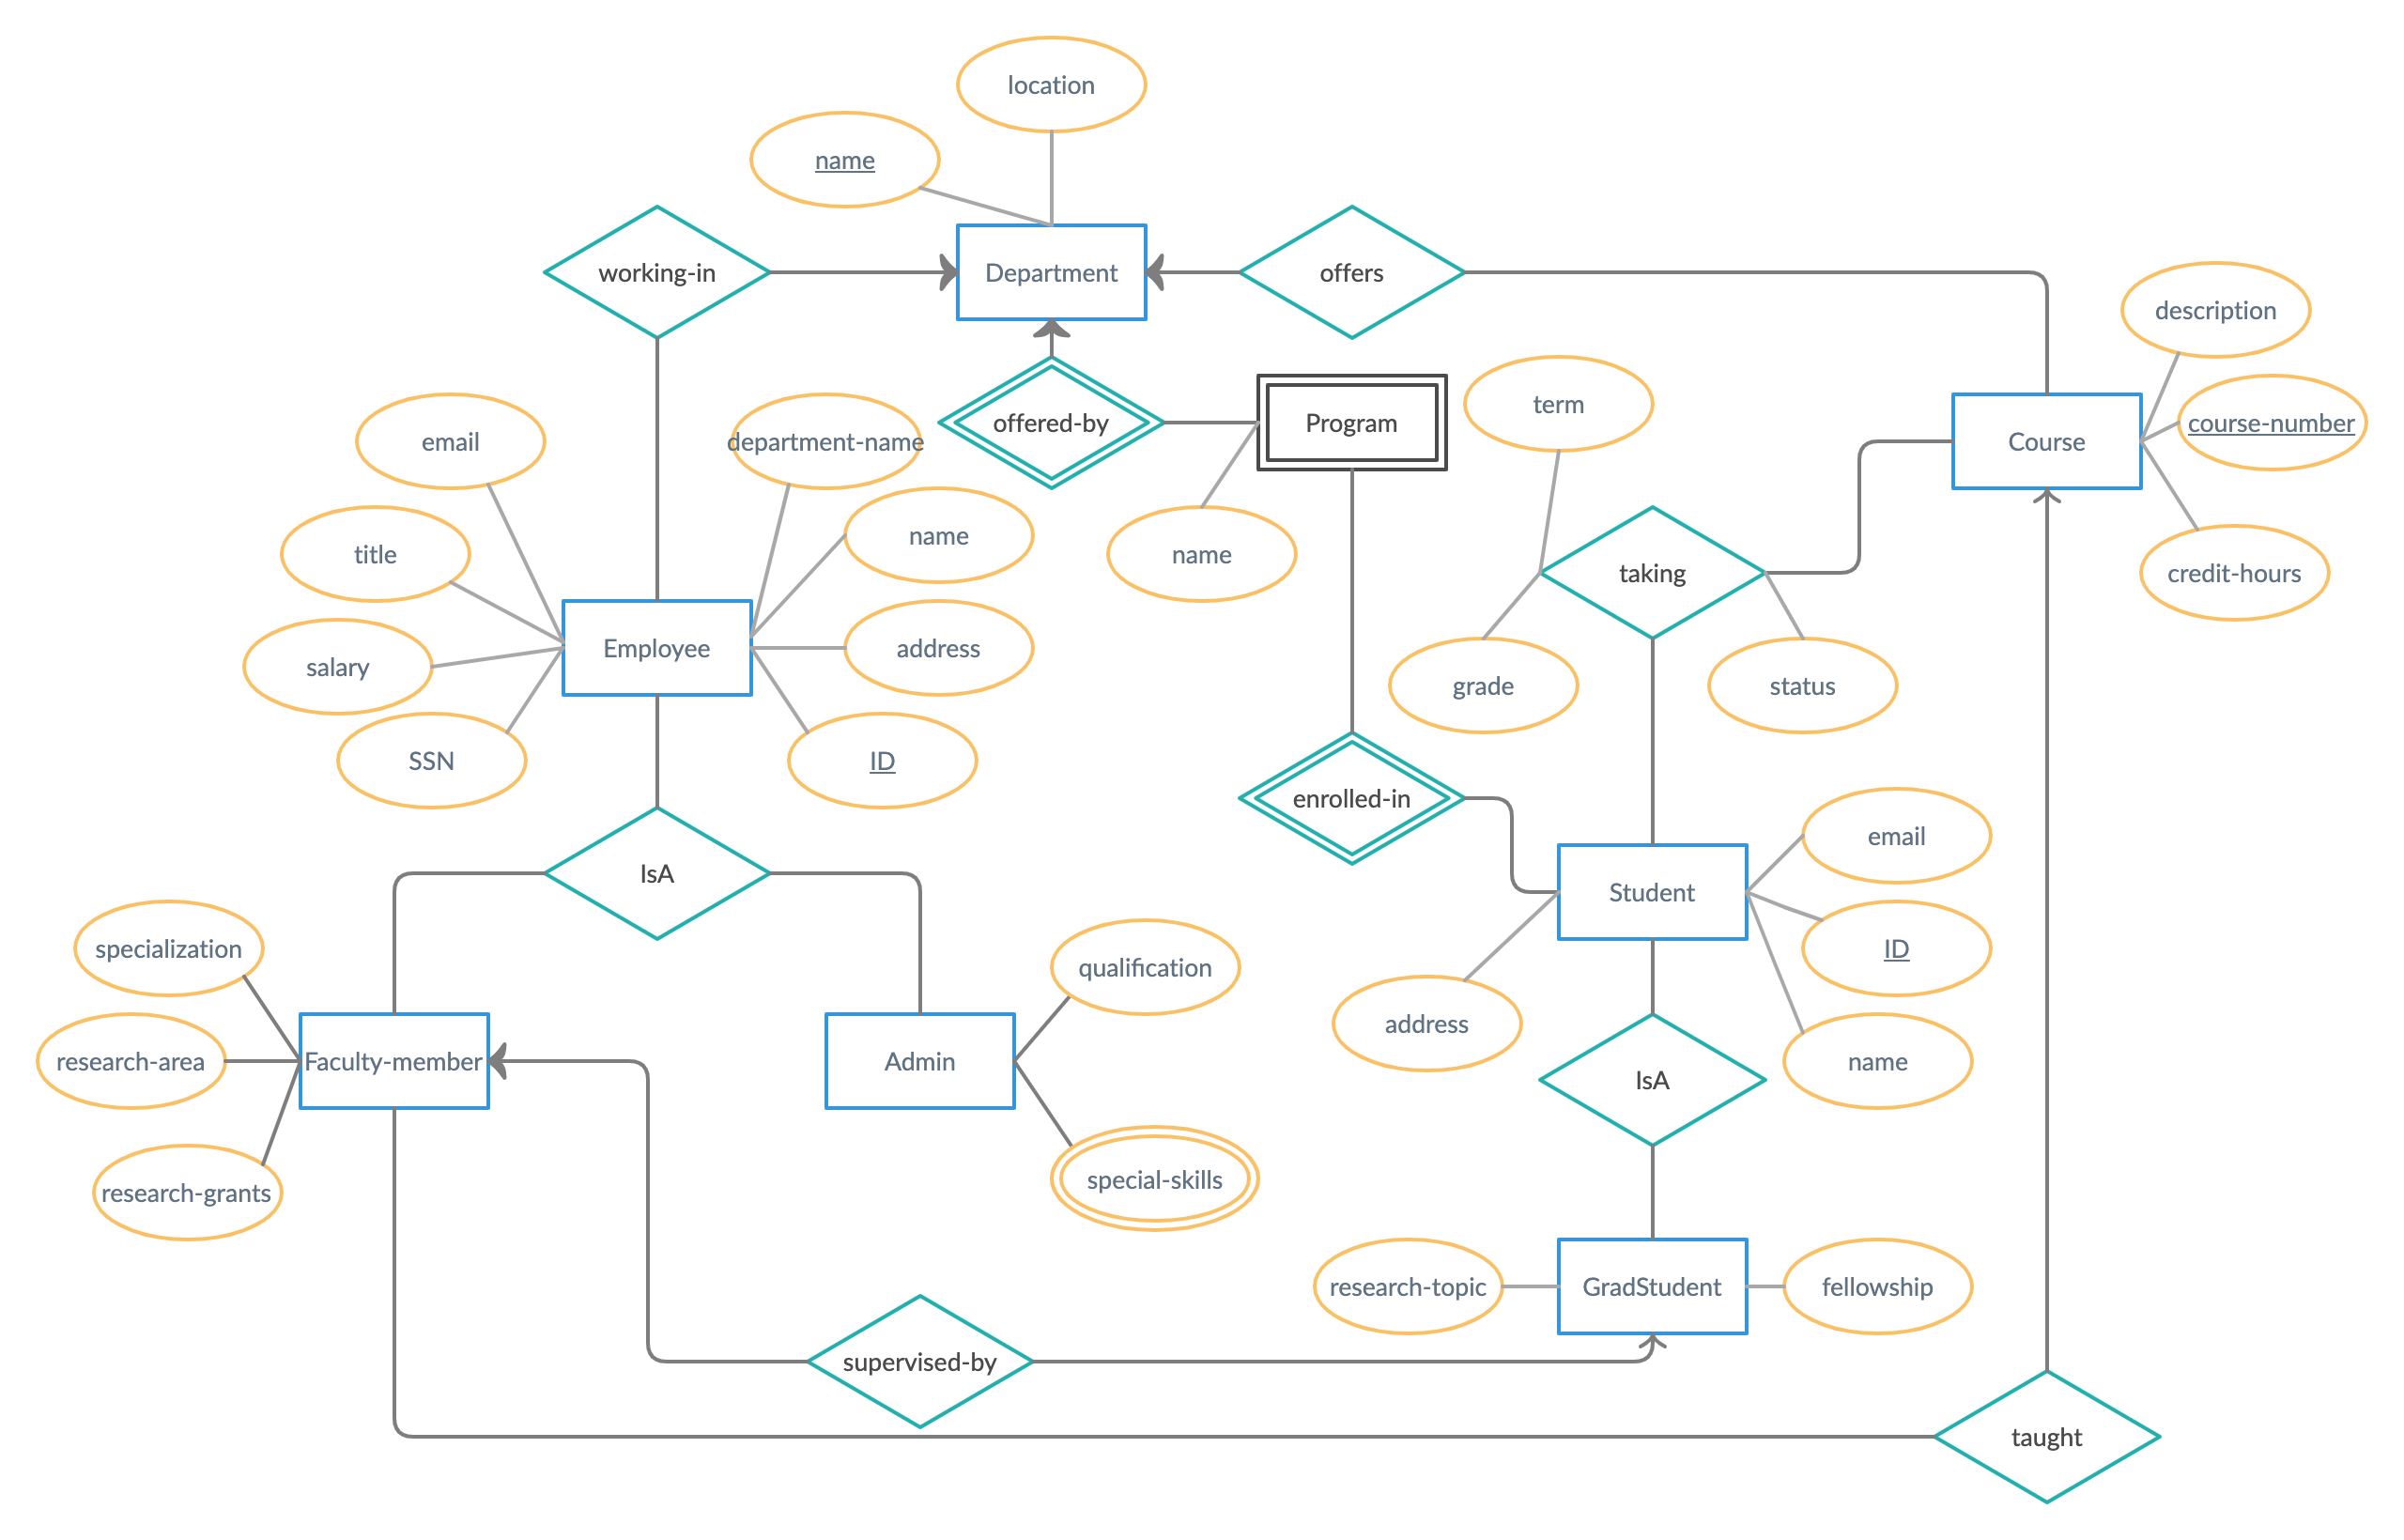
\includegraphics[scale=0.18]{ERD}
\centering
\end{figure}
\textit{Consult the file \textbf{ERD.png} in folder \textbf{./images} for a bigger version of the diagram}


\subsection{Mark the constraints}%
\label{sub:mark_the_constraints}

\textbf{Problem:}
In the diagram, mark the various constraints (keys, cardinalities of the relationships,
etc.). Identify any constraints that are not captured by the ER diagram.

\textbf{Constraints:}
\begin{itemize}
    \item The entity \textbf{Program} is not a requirement, but it was created to accommodate the need of enrolling students in \textbf{Student} entity and the need to keep track of programs offering by \textbf{Department} entity.
\end{itemize}

\newpage
\subsection{Convert ER diagram into relational database scheme}%
\label{sub:convert_er_diagraminto_relational_database_scheme}

\textbf{Problem:}
Convert your ER diagram into a relational database scheme. Make refinements to your
scheme if possible. Identify the primary keys and the foreign keys in the relational
schemes, and hence note the referential integrity constraints in the scheme.
\bigbreak
\begin{itemize}
    \item Department (\textcolor{red}{\underline{name}}, location)

    \item Employee (\textcolor{blue} {\underline{ID} }, address, name, \textcolor{red}{department-name}, email, title, salary, SSN)
    \item Faculty-member (\textcolor{blue}{\underline{ID}}, specialization, research-area, research-grants)
    \item Admin (\textcolor{blue} {\underline{ID}}, qualification)
    \item Special-skills (\textcolor{blue}{\underline{adminID}}, special-skill)

    \item Student (\textcolor{purple}{\underline{ID}}, name, address, email)
    \item taking (\textcolor{purple}{StudentID}, grade, status, term, \textcolor{cyan}{course-number})
    \item GradStudent (\textcolor{purple}{\underline{ID}}, fellowship, research-topic)
    \item supervised-by (\textcolor{blue}{FacultyID}, \textcolor{purple}{GradStuID})
    \item Program (name, \textcolor{red}{department-name}, \textcolor{purple}{studentID})

    \item Course (\textcolor{cyan}{\underline{course-number}}, description, credit-hours)
    \item taught (\textcolor{blue}{facultyMemberID}, \textcolor{cyan}{course-number})
    \item offers (\textcolor{red}{department-name}, \textcolor{cyan}{course-number})

\end{itemize}

\newpage 
\section{Question 2 [Marks 50]}

\subsection{Problem:}
Consider a DB schema consisting of the following relation schemes:
\begin{itemize}
    \item Patient (pid, pname, age, city)
    \item Doctor (did, dname, city)
    \item Specialization (did, specialization, start\_date\_of\_specialization)
    \item Clinic (cid, cname, city)
    \item Works\_in (did, cid, hours\_per\_week)
    \item Consults (pid, did, cid, date, illness)
\end{itemize}

\subsection{Express the queries in SQL}

\subsubsection{Get the detail (ID, doctor name and city) of doctors who are specialized in at least two
different specialization.}

\begin{verbatim}
SELECT Doctor.did, Doctor.dname, Doctor.city
FROM Doctor, Specialization
WHERE Doctor.did = Specialization.did
GROUP BY  Doctor.did
HAVING COUNT(distinct specialization) >= 2;
\end{verbatim}

\subsubsection{For a given patient, get the list of all the illnesses he has consulted for between given
dates.}

\begin{verbatim}
SELECT Patient.pname, Consults.illness
FROM Patient, Consults
WHERE Patient.pid = Consults.pid AND Patient.pname = "John"
AND Consults.date > "2020-05-19" AND Consults.date < "2020-10-22";
\end{verbatim}
\textbf{Note:}
\begin{itemize}
    \item This query is intended to get the list of all the illnesses a patient has consulted based on the name of the patient (eg: John). 
    \item The dates in the query serves as example only.
\end{itemize}

\subsubsection{Give a list of patients name and the doctors name where the patient consulted the doctor
in clinics in the cities of Montreal and Laval between January first of 2020 and march 15
of 2020 and the illness was assigned to be “High Fever”.}

\begin{verbatim}
SELECT Patient.pname, Doctor.dname
FROM Patient, Doctor, Consults, Clinic
WHERE Patient.pid = Consults.pid AND Doctor.did = Consults.did
AND Consults.cid = Clinic.cid AND (Clinic.city = "Montreal" OR Clinic.city = "Laval") 
AND Consults.date >= "2020-01-01" AND Consults.date <= "2020-03-15"
AND Consults.illness = "High Fever";
\end{verbatim}

\subsubsection{Give details of patients who have consulted Dr. Roberto at least twice}
\begin{verbatim}
SELECT Patient.pid, Patient.pname, Patient.age, Patient.city 
FROM Patient, Doctor, Consults
WHERE Doctor.dname = "Roberto"
AND Consults.did = Doctor.did AND Patient.pid = Consults.pid
GROUP BY Patient.pid
HAVING COUNT(Consults.pid) >= 2;
\end{verbatim}

\subsubsection{Give details of doctors who work in clinics in “Laval” but have never worked in clinics
in “West Island”.}
\begin{verbatim}
SELECT Doctor.did, Doctor.dname, Doctor.city
FROM Doctor, Works_in, Clinic
WHERE Doctor.did = Works_in.did AND Clinic.cid = Works_in.cid 
AND Clinic.city = "Laval" AND Doctor.did NOT IN (
SELECT Doctor.did
FROM Doctor, Works_in, Clinic
WHERE Doctor.did = Works_in.did AND Clinic.cid = Works_in.cid 
AND Clinic.city = "West Island"
);
\end{verbatim}


\subsubsection{Give the name and city of doctors who work at least a total of 60 hours a week whether
in the same clinic or in more than one clinic.}
\begin{verbatim}
SELECT Doctor.dname, Doctor.city 
FROM Doctor, Works_in
WHERE Doctor.did = Works_in.did
GROUP BY Doctor.did
HAVING SUM(hours_per_week) >= 60;
\end{verbatim}

\end{document}
